% !TeX encoding = UTF-8
% !TeX spellcheck = uk_UA
% !Mode:: "TeX:ACP"
\documentclass{KnuBulletin}

%% LaTeX/XeTeX шаблон для статтей у Вісник Київського національного університету імені Тараса Шевченка, 
%% Серія фізико-математичні науки.
%% 
%% Остання версія шаблону завжди тут: https://github.com/ertong/knu-bulletin
%% 
%% Автор: Ігор Литвиненко

\begin{document}

% Вказуємо рік  та номер виданння
\yearNumber{2014}{1}

% Вказуємо дату подачі до друку
\submittedDate{09.01.14}

% Вказуємо авторів. Цей блок повторюється для кожного автора.
% вказуючи науковий ступінь та вчене звання, 
% використовуйте такі скорочення: 
% д.ф.-м.н., к.ф.-м.н., проф., доц., асист., пров.н.с., с.н.с., 
% м.н.с., д.т.н, к.т.н, аспірант, студент
\author
{І. O. Іваненко} %Ініціали та прізвище
{аспірант} % науковий ступінь та вчене звання
{Київський національний університет імені Тараса Шевченка, 03680, м. Київ, пр-т Глушкова 4д} % назва та адреса установи
{I. O. Ivanenko}
{PhD student}
{Taras Shevchenko National University of Kyiv, 03680, Kyiv, Glushkova av., 4d}
{ivan@example.ua} % електронна адреса

\author
{І. І. Петренко}
{д.ф.-м.н., проф.}
{Київський національний університет імені Тараса Шевченка, 03680, м. Київ, пр-т Глушкова 4д}
{I. I. Petrenko}
{Doctor of Sciences, Full Professor}
{Taras Shevchenko National University of Kyiv, 03680, Kyiv, Glushkova av., 4d}
{petro@example.ua}

\header
{519.21} %УДК
% Назва статті українською мовою
{Зразок оформлення статті}
% Аннотація українською мовою
{
    Тут розміщується анотація до статті українською мовою.
    
    Текст анотації може містити декілька абзаців, що 
    коротко описують зміст роботи.
}
% ключові слова (від 3-х до 10-ти штук)
{система обслуговування, рекурентний потік, стаціонарні ймовірності}
% теж саме англійською мовою
{Paper template}
{
	This is an abstract to your paper. English version should be written here.
	
	Abstract can have several paragraphs, which shortly describe your paper.
}
{queuing system, recurrent flow, stationary probabilities}

%статтю може представляти лише член редколегії журналу
Статтю представив д.ф.-м.н., проф. Сидоренко М.М. 

\begin{multicols}{2}
    \noindent % перших параграф не має відступу
    
    Тут починається текст статті для журналу ''Вісник Київського національного університету імені Тараса Шевченка. Серія фізико-математичні науки``. 

	Разом з статтею подається інформація про неї для надання даних в УРЖ ''Джерело`` у форматі MS Word 97/2003/2007/2010 до редколегії, роздрукована на білому папері формату А4 разом із електронною копією. Крім цього необхідно подати рецензію на статтю та виписку з протоколу засідання кафедри, на якому робота була рекомендована до друку у журналі. Усі тверді копії подаються в одному екземплярі.
    Робота може бути подана українською або англійською мовами. Прізвища авторів, назва роботи, резюме та ключові слова оформляються згідно наведеного зразка українською та англійською мовою.
\end{multicols}

\begin{table}[H]
\centering % The table will be centered
\caption{Таблиця, розміщена на всю ширину сторінки} % the table signature
\label{tab-1} % we are specifying the table name; it is used for autonumbering and references
\begin{tabular}{|c|c|c|c|c|c|c|}
\hline
Колонка 1& Колонка 2& Колонка 3& Колонка 4& Колонка 5& Колонка 6 & Колонка 7\\
\hline
&&&&&&\\
\hline
&&&&&&\\
\hline
&&&&&&\\
\hline
\end{tabular}
\end{table}

\begin{multicols}{2}
		 \begin{figure}[H]
		     \hfil
		     % This file was created by matlab2tikz v0.3.3.
% Copyright (c) 2008--2013, Nico Schlömer <nico.schloemer@gmail.com>
% All rights reserved.
% 
% The latest updates can be retrieved from
%   http://www.mathworks.com/matlabcentral/fileexchange/22022-matlab2tikz
% where you can also make suggestions and rate matlab2tikz.
% 
% 
% 
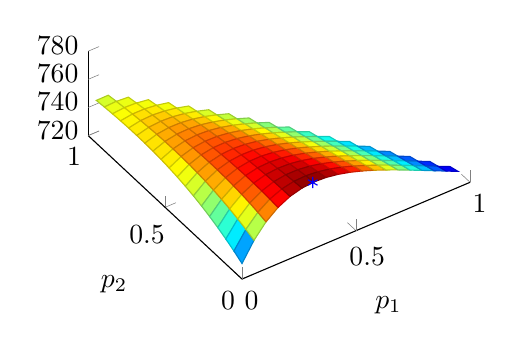
\begin{tikzpicture}

\begin{axis}[%
width=0.4\textwidth,
height=0.34\textwidth,
unbounded coords=jump,
view={-34}{64},
scale only axis,
xmin=0,
xmax=1,
xlabel={$p_1$},
ymin=0,
ymax=1,
ylabel={$p_2$},
zmin=720,
zmax=780,
title={},
axis x line*=bottom,
axis y line*=left,
axis z line*=left
]

\addplot3[%
surf,
colormap/jet,
shader=faceted,
draw=black,
mesh/rows=20]
table[row sep=crcr,header=false] {
0 0 731.013477419278\\
0 0.0526315789473684 734.563492038168\\
0 0.105263157894737 737.729408392122\\
0 0.157894736842105 740.528468106508\\
0 0.210526315789474 742.978554038338\\
0 0.263157894736842 745.09789642451\\
0 0.315789473684211 746.904825958476\\
0 0.368421052631579 748.417569122293\\
0 0.421052631578947 749.654081141013\\
0 0.473684210526316 750.631912084126\\
0 0.526315789473684 751.368101880567\\
0 0.578947368421053 751.879100311183\\
0 0.631578947368421 752.180708372434\\
0 0.684210526315789 752.288037749064\\
0 0.736842105263158 752.215485477769\\
0 0.789473684210526 751.976721218005\\
0 0.842105263157895 751.584684863127\\
0 0.894736842105263 751.051592520235\\
0 0.947368421052632 750.388949157829\\
0 1 749.607566465488\\
0.0526315789473684 0 743.913171185566\\
0.0526315789473684 0.0526315789473684 746.315283932909\\
0.0526315789473684 0.105263157894737 748.388322245117\\
0.0526315789473684 0.157894736842105 750.150557819217\\
0.0526315789473684 0.210526315789474 751.620150968364\\
0.0526315789473684 0.263157894736842 752.814986281177\\
0.0526315789473684 0.315789473684211 753.752540898407\\
0.0526315789473684 0.368421052631579 754.449781247862\\
0.0526315789473684 0.421052631578947 754.923084370203\\
0.0526315789473684 0.473684210526316 755.188180291501\\
0.0526315789473684 0.526315789473684 755.260112235672\\
0.0526315789473684 0.578947368421053 755.153211807271\\
0.0526315789473684 0.631578947368421 754.881086602822\\
0.0526315789473684 0.684210526315789 754.456618019832\\
0.0526315789473684 0.736842105263158 753.891967322244\\
0.0526315789473684 0.789473684210526 753.198588286934\\
0.0526315789473684 0.842105263157895 752.387244996573\\
0.0526315789473684 0.894736842105263 751.468033559872\\
0.0526315789473684 0.947368421052632 750.450406731602\\
0.0526315789473684 1 Inf\\
0.105263157894737 0 753.409380564311\\
0.105263157894737 0.0526315789473684 754.834848575162\\
0.105263157894737 0.105263157894737 755.987076733252\\
0.105263157894737 0.157894736842105 756.883470859558\\
0.105263157894737 0.210526315789474 757.540924609301\\
0.105263157894737 0.263157894736842 757.9757423033\\
0.105263157894737 0.315789473684211 758.203582455857\\
0.105263157894737 0.368421052631579 758.239418850639\\
0.105263157894737 0.421052631578947 758.097516346414\\
0.105263157894737 0.473684210526316 757.791418915431\\
0.105263157894737 0.526315789473684 757.333947721857\\
0.105263157894737 0.578947368421053 756.737207331604\\
0.105263157894737 0.631578947368421 756.012598405466\\
0.105263157894737 0.684210526315789 755.170835463672\\
0.105263157894737 0.736842105263158 754.221968521654\\
0.105263157894737 0.789473684210526 753.175407584744\\
0.105263157894737 0.842105263157895 752.039949154881\\
0.105263157894737 0.894736842105263 750.823804046816\\
0.105263157894737 0.947368421052632 Inf\\
0.105263157894737 1 Inf\\
0.157894736842105 0 760.025520507465\\
0.157894736842105 0.0526315789473684 760.642309621724\\
0.157894736842105 0.105263157894737 761.037811768447\\
0.157894736842105 0.157894736842105 761.227613636655\\
0.157894736842105 0.210526315789474 761.226618759984\\
0.157894736842105 0.263157894736842 761.04902405895\\
0.157894736842105 0.315789473684211 760.708308401317\\
0.157894736842105 0.368421052631579 760.217231028797\\
0.157894736842105 0.421052631578947 759.587837976169\\
0.157894736842105 0.473684210526316 758.831474864116\\
0.157894736842105 0.526315789473684 757.958804678408\\
0.157894736842105 0.578947368421053 756.979829355574\\
0.157894736842105 0.631578947368421 755.903914179461\\
0.157894736842105 0.684210526315789 754.739814155319\\
0.157894736842105 0.736842105263158 753.495701669827\\
0.157894736842105 0.789473684210526 752.179194868389\\
0.157894736842105 0.842105263157895 750.797386286963\\
0.157894736842105 0.894736842105263 Inf\\
0.157894736842105 0.947368421052632 Inf\\
0.157894736842105 1 Inf\\
0.210526315789474 0 764.261011630062\\
0.210526315789474 0.0526315789473684 764.222410079989\\
0.210526315789474 0.105263157894737 764.008394842627\\
0.210526315789474 0.157894736842105 763.632378290111\\
0.210526315789474 0.210526315789474 763.107056106864\\
0.210526315789474 0.263157894736842 762.444413989388\\
0.210526315789474 0.315789473684211 761.655740597323\\
0.210526315789474 0.368421052631579 760.751645394874\\
0.210526315789474 0.421052631578947 759.74208022469\\
0.210526315789474 0.473684210526316 758.636363636759\\
0.210526315789474 0.526315789473684 757.443207153784\\
0.210526315789474 0.578947368421053 756.170742793436\\
0.210526315789474 0.631578947368421 754.826551288446\\
0.210526315789474 0.684210526315789 753.417690549422\\
0.210526315789474 0.736842105263158 751.95072400427\\
0.210526315789474 0.789473684210526 750.431748523806\\
0.210526315789474 0.842105263157895 Inf\\
0.210526315789474 0.894736842105263 Inf\\
0.210526315789474 0.947368421052632 Inf\\
0.210526315789474 1 Inf\\
0.263157894736842 0 766.564287743779\\
0.263157894736842 0.0526315789473684 766.004044958114\\
0.263157894736842 0.105263157894737 765.307521938997\\
0.263157894736842 0.157894736842105 764.485948467819\\
0.263157894736842 0.210526315789474 763.549878484692\\
0.263157894736842 0.263157894736842 762.509211692925\\
0.263157894736842 0.315789473684211 761.373217854162\\
0.263157894736842 0.368421052631579 760.150562971807\\
0.263157894736842 0.421052631578947 758.849336696313\\
0.263157894736842 0.473684210526316 757.477080403912\\
0.263157894736842 0.526315789473684 756.04081550215\\
0.263157894736842 0.578947368421053 754.547071602796\\
0.263157894736842 0.631578947368421 753.001914276959\\
0.263157894736842 0.684210526315789 751.410972170057\\
0.263157894736842 0.736842105263158 749.779463307127\\
0.263157894736842 0.789473684210526 Inf\\
0.263157894736842 0.842105263157895 Inf\\
0.263157894736842 0.894736842105263 Inf\\
0.263157894736842 0.947368421052632 Inf\\
0.263157894736842 1 Inf\\
0.315789473684211 0 767.322683942097\\
0.315789473684211 0.0526315789473684 766.354055408307\\
0.315789473684211 0.105263157894737 765.281743009781\\
0.315789473684211 0.157894736842105 764.114965619516\\
0.315789473684211 0.210526315789474 762.862341630027\\
0.315789473684211 0.263157894736842 761.531916264914\\
0.315789473684211 0.315789473684211 760.1311895341\\
0.315789473684211 0.368421052631579 758.66714439548\\
0.315789473684211 0.421052631578947 757.146274771053\\
0.315789473684211 0.473684210526316 755.574613138236\\
0.315789473684211 0.526315789473684 753.95775747859\\
0.315789473684211 0.578947368421053 752.300897417921\\
0.315789473684211 0.631578947368421 750.608839434991\\
0.315789473684211 0.684210526315789 748.886031051945\\
0.315789473684211 0.736842105263158 Inf\\
0.315789473684211 0.789473684210526 Inf\\
0.315789473684211 0.842105263157895 Inf\\
0.315789473684211 0.894736842105263 Inf\\
0.315789473684211 0.947368421052632 Inf\\
0.315789473684211 1 Inf\\
0.368421052631579 0 766.862125010563\\
0.368421052631579 0.0526315789473684 765.579030561661\\
0.368421052631579 0.105263157894737 764.21894003708\\
0.368421052631579 0.157894736842105 762.789309998627\\
0.368421052631579 0.210526315789474 761.297082933231\\
0.368421052631579 0.263157894736842 759.748715123388\\
0.368421052631579 0.315789473684211 758.150204082487\\
0.368421052631579 0.368421052631579 756.507115342442\\
0.368421052631579 0.421052631578947 754.824608431576\\
0.368421052631579 0.473684210526316 753.107461923022\\
0.368421052631579 0.526315789473684 751.360097469014\\
0.368421052631579 0.578947368421053 749.58660276538\\
0.368421052631579 0.631578947368421 747.790753414194\\
0.368421052631579 0.684210526315789 Inf\\
0.368421052631579 0.736842105263158 Inf\\
0.368421052631579 0.789473684210526 Inf\\
0.368421052631579 0.842105263157895 Inf\\
0.368421052631579 0.894736842105263 Inf\\
0.368421052631579 0.947368421052632 Inf\\
0.368421052631579 1 Inf\\
0.421052631578947 0 765.451899251998\\
0.421052631578947 0.0526315789473684 763.931061240283\\
0.421052631578947 0.105263157894737 762.354797094606\\
0.421052631578947 0.157894736842105 760.72906741059\\
0.421052631578947 0.210526315789474 759.05940340232\\
0.421052631578947 0.263157894736842 757.350932721679\\
0.421052631578947 0.315789473684211 755.608404348222\\
0.421052631578947 0.368421052631579 753.83621246762\\
0.421052631578947 0.421052631578947 752.038419284904\\
0.421052631578947 0.473684210526316 750.21877674189\\
0.421052631578947 0.526315789473684 748.380747126828\\
0.421052631578947 0.578947368421053 746.527522579305\\
0.421052631578947 0.631578947368421 Inf\\
0.421052631578947 0.684210526315789 Inf\\
0.421052631578947 0.736842105263158 Inf\\
0.421052631578947 0.789473684210526 Inf\\
0.421052631578947 0.842105263157895 Inf\\
0.421052631578947 0.894736842105263 Inf\\
0.421052631578947 0.947368421052632 Inf\\
0.421052631578947 1 Inf\\
0.473684210526316 0 763.311606637578\\
0.473684210526316 0.0526315789473684 761.615000969919\\
0.473684210526316 0.105263157894737 759.880226895884\\
0.473684210526316 0.157894736842105 758.112002027706\\
0.473684210526316 0.210526315789474 756.314691405135\\
0.473684210526316 0.263157894736842 754.492330156797\\
0.473684210526316 0.315789473684211 752.648645070735\\
0.473684210526316 0.368421052631579 750.787075063362\\
0.473684210526316 0.421052631578947 748.910790550644\\
0.473684210526316 0.473684210526316 747.02271173688\\
0.473684210526316 0.526315789473684 745.125525845375\\
0.473684210526316 0.578947368421053 Inf\\
0.473684210526316 0.631578947368421 Inf\\
0.473684210526316 0.684210526315789 Inf\\
0.473684210526316 0.736842105263158 Inf\\
0.473684210526316 0.789473684210526 Inf\\
0.473684210526316 0.842105263157895 Inf\\
0.473684210526316 0.894736842105263 Inf\\
0.473684210526316 0.947368421052632 Inf\\
0.473684210526316 1 Inf\\
0.526315789473684 0 760.618610838424\\
0.526315789473684 0.0526315789473684 758.795868822352\\
0.526315789473684 0.105263157894737 756.948649934408\\
0.526315789473684 0.157894736842105 755.080654232404\\
0.526315789473684 0.210526315789474 753.195295778277\\
0.526315789473684 0.263157894736842 751.295721872575\\
0.526315789473684 0.315789473684211 749.384831213522\\
0.526315789473684 0.368421052631579 747.465291005362\\
0.526315789473684 0.421052631578947 745.53955304725\\
0.526315789473684 0.473684210526316 743.609868838847\\
0.526315789473684 0.526315789473684 Inf\\
0.526315789473684 0.578947368421053 Inf\\
0.526315789473684 0.631578947368421 Inf\\
0.526315789473684 0.684210526315789 Inf\\
0.526315789473684 0.736842105263158 Inf\\
0.526315789473684 0.789473684210526 Inf\\
0.526315789473684 0.842105263157895 Inf\\
0.526315789473684 0.894736842105263 Inf\\
0.526315789473684 0.947368421052632 Inf\\
0.526315789473684 1 Inf\\
0.578947368421053 0 757.515118236262\\
0.578947368421053 0.0526315789473684 755.605704526478\\
0.578947368421053 0.105263157894737 753.682594245379\\
0.578947368421053 0.157894736842105 751.748663203464\\
0.578947368421053 0.210526315789474 749.806557292443\\
0.578947368421053 0.263157894736842 747.858708455237\\
0.578947368421053 0.315789473684211 745.907349680102\\
0.578947368421053 0.368421052631579 743.954529058374\\
0.578947368421053 0.421052631578947 742.002122947582\\
0.578947368421053 0.473684210526316 Inf\\
0.578947368421053 0.526315789473684 Inf\\
0.578947368421053 0.578947368421053 Inf\\
0.578947368421053 0.631578947368421 Inf\\
0.578947368421053 0.684210526315789 Inf\\
0.578947368421053 0.736842105263158 Inf\\
0.578947368421053 0.789473684210526 Inf\\
0.578947368421053 0.842105263157895 Inf\\
0.578947368421053 0.894736842105263 Inf\\
0.578947368421053 0.947368421052632 Inf\\
0.578947368421053 1 Inf\\
0.631578947368421 0 754.114485033053\\
0.631578947368421 0.0526315789473684 752.149585574553\\
0.631578947368421 0.105263157894737 750.179415014986\\
0.631578947368421 0.157894736842105 748.206186631422\\
0.631578947368421 0.210526315789474 746.231930124852\\
0.631578947368421 0.263157894736842 744.258504681904\\
0.631578947368421 0.315789473684211 742.287611191856\\
0.631578947368421 0.368421052631579 740.320803662086\\
0.631578947368421 0.421052631578947 Inf\\
0.631578947368421 0.473684210526316 Inf\\
0.631578947368421 0.526315789473684 Inf\\
0.631578947368421 0.578947368421053 Inf\\
0.631578947368421 0.631578947368421 Inf\\
0.631578947368421 0.684210526315789 Inf\\
0.631578947368421 0.736842105263158 Inf\\
0.631578947368421 0.789473684210526 Inf\\
0.631578947368421 0.842105263157895 Inf\\
0.631578947368421 0.894736842105263 Inf\\
0.631578947368421 0.947368421052632 Inf\\
0.631578947368421 1 Inf\\
0.684210526315789 0 750.506624934947\\
0.684210526315789 0.0526315789473684 748.510737750295\\
0.684210526315789 0.105263157894737 746.516112750537\\
0.684210526315789 0.157894736842105 744.524433743578\\
0.684210526315789 0.210526315789474 742.537238764236\\
0.684210526315789 0.263157894736842 740.555930645649\\
0.684210526315789 0.315789473684211 738.581786880812\\
0.684210526315789 0.368421052631579 Inf\\
0.684210526315789 0.421052631578947 Inf\\
0.684210526315789 0.473684210526316 Inf\\
0.684210526315789 0.526315789473684 Inf\\
0.684210526315789 0.578947368421053 Inf\\
0.684210526315789 0.631578947368421 Inf\\
0.684210526315789 0.684210526315789 Inf\\
0.684210526315789 0.736842105263158 Inf\\
0.684210526315789 0.789473684210526 Inf\\
0.684210526315789 0.842105263157895 Inf\\
0.684210526315789 0.894736842105263 Inf\\
0.684210526315789 0.947368421052632 Inf\\
0.684210526315789 1 Inf\\
0.736842105263158 0 746.762533139808\\
0.736842105263158 0.0526315789473684 744.754783930205\\
0.736842105263158 0.105263157894737 742.75331718554\\
0.736842105263158 0.157894736842105 740.759395503213\\
0.736842105263158 0.210526315789474 738.774166266712\\
0.736842105263158 0.263157894736842 736.798670137777\\
0.736842105263158 0.315789473684211 Inf\\
0.736842105263158 0.368421052631579 Inf\\
0.736842105263158 0.421052631578947 Inf\\
0.736842105263158 0.473684210526316 Inf\\
0.736842105263158 0.526315789473684 Inf\\
0.736842105263158 0.578947368421053 Inf\\
0.736842105263158 0.631578947368421 Inf\\
0.736842105263158 0.684210526315789 Inf\\
0.736842105263158 0.736842105263158 Inf\\
0.736842105263158 0.789473684210526 Inf\\
0.736842105263158 0.842105263157895 Inf\\
0.736842105263158 0.894736842105263 Inf\\
0.736842105263158 0.947368421052632 Inf\\
0.736842105263158 1 Inf\\
0.789473684210526 0 742.938009892573\\
0.789473684210526 0.0526315789473684 740.933226447307\\
0.789473684210526 0.105263157894737 738.938540465698\\
0.789473684210526 0.157894736842105 736.954880726041\\
0.789473684210526 0.210526315789474 734.983085339572\\
0.789473684210526 0.263157894736842 Inf\\
0.789473684210526 0.315789473684211 Inf\\
0.789473684210526 0.368421052631579 Inf\\
0.789473684210526 0.421052631578947 Inf\\
0.789473684210526 0.473684210526316 Inf\\
0.789473684210526 0.526315789473684 Inf\\
0.789473684210526 0.578947368421053 Inf\\
0.789473684210526 0.631578947368421 Inf\\
0.789473684210526 0.684210526315789 Inf\\
0.789473684210526 0.736842105263158 Inf\\
0.789473684210526 0.789473684210526 Inf\\
0.789473684210526 0.842105263157895 Inf\\
0.789473684210526 0.894736842105263 Inf\\
0.789473684210526 0.947368421052632 Inf\\
0.789473684210526 1 Inf\\
0.842105263157895 0 739.076691778449\\
0.842105263157895 0.0526315789473684 737.086273934117\\
0.842105263157895 0.105263157894737 735.108811326858\\
0.842105263157895 0.157894736842105 733.144969080878\\
0.842105263157895 0.210526315789474 Inf\\
0.842105263157895 0.263157894736842 Inf\\
0.842105263157895 0.315789473684211 Inf\\
0.842105263157895 0.368421052631579 Inf\\
0.842105263157895 0.421052631578947 Inf\\
0.842105263157895 0.473684210526316 Inf\\
0.842105263157895 0.526315789473684 Inf\\
0.842105263157895 0.578947368421053 Inf\\
0.842105263157895 0.631578947368421 Inf\\
0.842105263157895 0.684210526315789 Inf\\
0.842105263157895 0.736842105263158 Inf\\
0.842105263157895 0.789473684210526 Inf\\
0.842105263157895 0.842105263157895 Inf\\
0.842105263157895 0.894736842105263 Inf\\
0.842105263157895 0.947368421052632 Inf\\
0.842105263157895 1 Inf\\
0.894736842105263 0 735.212501240476\\
0.894736842105263 0.0526315789473684 733.245121221084\\
0.894736842105263 0.105263157894737 731.292796025648\\
0.894736842105263 0.157894736842105 Inf\\
0.894736842105263 0.210526315789474 Inf\\
0.894736842105263 0.263157894736842 Inf\\
0.894736842105263 0.315789473684211 Inf\\
0.894736842105263 0.368421052631579 Inf\\
0.894736842105263 0.421052631578947 Inf\\
0.894736842105263 0.473684210526316 Inf\\
0.894736842105263 0.526315789473684 Inf\\
0.894736842105263 0.578947368421053 Inf\\
0.894736842105263 0.631578947368421 Inf\\
0.894736842105263 0.684210526315789 Inf\\
0.894736842105263 0.736842105263158 Inf\\
0.894736842105263 0.789473684210526 Inf\\
0.894736842105263 0.842105263157895 Inf\\
0.894736842105263 0.894736842105263 Inf\\
0.894736842105263 0.947368421052632 Inf\\
0.894736842105263 1 Inf\\
0.947368421052632 0 731.37161621839\\
0.947368421052632 0.0526315789473684 729.433780247607\\
0.947368421052632 0.105263157894737 Inf\\
0.947368421052632 0.157894736842105 Inf\\
0.947368421052632 0.210526315789474 Inf\\
0.947368421052632 0.263157894736842 Inf\\
0.947368421052632 0.315789473684211 Inf\\
0.947368421052632 0.368421052631579 Inf\\
0.947368421052632 0.421052631578947 Inf\\
0.947368421052632 0.473684210526316 Inf\\
0.947368421052632 0.526315789473684 Inf\\
0.947368421052632 0.578947368421053 Inf\\
0.947368421052632 0.631578947368421 Inf\\
0.947368421052632 0.684210526315789 Inf\\
0.947368421052632 0.736842105263158 Inf\\
0.947368421052632 0.789473684210526 Inf\\
0.947368421052632 0.842105263157895 Inf\\
0.947368421052632 0.894736842105263 Inf\\
0.947368421052632 0.947368421052632 Inf\\
0.947368421052632 1 Inf\\
1 0 727.574048850582\\
1 0.0526315789473684 Inf\\
1 0.105263157894737 Inf\\
1 0.157894736842105 Inf\\
1 0.210526315789474 Inf\\
1 0.263157894736842 Inf\\
1 0.315789473684211 Inf\\
1 0.368421052631579 Inf\\
1 0.421052631578947 Inf\\
1 0.473684210526316 Inf\\
1 0.526315789473684 Inf\\
1 0.578947368421053 Inf\\
1 0.631578947368421 Inf\\
1 0.684210526315789 Inf\\
1 0.736842105263158 Inf\\
1 0.789473684210526 Inf\\
1 0.842105263157895 Inf\\
1 0.894736842105263 Inf\\
1 0.947368421052632 Inf\\
1 1 Inf\\
};
\addplot3 [
color=blue,
only marks,
mark=asterisk,
mark options={solid}]
table[row sep=crcr] {
0.310167892279534 7.35675409480052e-13 767.305066768755\\
};
\end{axis}
\end{tikzpicture}%
		     \hfil
		     \caption{Функція $\sum_{i=1}^{N} c_i \E{X^i}$ в залежності від $p$.}
		     \label{fig-1}
		 \end{figure}	
    
	Робота готується на білому папері формату А4 (210 мм х 297 мм). 
	
	Таблиці та ілюстрації вносяться безпосередньо в текст. 
	Їх слід розташовувати так, щоб вони осягали по ширині увесь текст (табл. \ref{tab-1}) 
	або одну колонку (рис. \ref{fig-1}). 
	Довгі виносні формули також рекомендується розташовувати по ширині двох колонок тексту. 

	Всі позначення та символи на рисунках повинні бути не менші 2.0 мм (5 pt) за розміром. Не слід використовувати занадто темних або занадто світлих рисунків чи сканованих фотографій. Товщина ліній на графіках та обрамлень у таблицях має бути не меншою 0.75pt (0.3 мм), також не варто лінії робити товщими 2pt (0.7 мм). Всі підписи на осях координат, на схемах і т.п. повинні бути мовою статті (тобто не допускаються англомовні підписи в роботах українською мовою). 
	
	Теореми, леми та наслідки оформлюються як лема \ref{lem-1}.
    \begin{lemma}
    	\label{lem-1}
	    Теореми, твердження, леми та наслідки оформляються в оточеннях 
	    \texttt{theorem}, \texttt{statement}, \texttt{lemma} та \texttt{corollary} відповідно.
    \end{lemma}
    \begin{proof}
    	Доведення оформляються в оточенні \texttt{proof}.
    \end{proof}

    \begin{definition}
	   	Означення оформляються в оточенні \texttt{definition}.
	\end{definition}	
    

	\begin{remark}
		Приклади та зауваження оформляються в оточеннях 
		\texttt{example} та \texttt{remark} відповідно.
	\end{remark}
	
	Якщо стаття поділена на підрозділи, заголовки потрібно оформляти наступним чином. 
	\section*{Підзаголовок}

	Список використаних джерел оформляється згідно вимог стандарту ГОСТ. 
	Він повинен закінчуватися в нижній третині сторінки/колонки основного тексту, щоб не залишалось незаповнене текстом велике поле в кінці статті. 
	
	Посилання у тексті роботи позначаються цифрами у квадратних дужках (наприклад, \cite{takacs1962} чи \cite{klimov1966}) та вказуються 
	виключно англійською мовою. 
	Посилатися на неопубліковані роботи не рекомендується. 


	% Посилання на джерела.
	% Будується автоматично, базуючись на згадуваннях
	% в тексті за допомогою \cite{book-name}.
	% 
	% Бібліографічна інформація знаходиться в example.bib
	% 
	% Всі посилання оформляються виключно англійською мовою.
    \bibliography{example}
    

\end{multicols}
\end{document}